\section{Gouvernance institutionnelle de l'IA}
\label{sec:6_axe5_gouvernance}

Les enquêtes nationales analysées dans la section précédente révèlent une adoption inégale de l'\gls{ia} générative : si 75\% des étudiants des Grandes Écoles l'utilisent régulièrement, seuls 52\% des enseignants-chercheurs franchissent le pas, freinés par le manque de formation (65\%) et l'absence de politique claire au sein de leurs établissements (44\%). Les écoles d'ingénieurs accusent un retard structurel préoccupant en matière de gouvernance : 55\% disposent d'une gouvernance \gls{ia} établie, contre 89\% des écoles de commerce~\cite{pascal2025ia,cge2024enquete}. Ces diagnostics individuels et disciplinaires appellent désormais un changement d'échelle : comment structurer l'émergence de ces technologies à l'échelle des établissements et des réseaux ? Quels modèles de gouvernance, quelles infrastructures souveraines, quelles stratégies de formation de masse permettent d'accompagner cette transformation ? L'écosystème français de l'enseignement supérieur a connu une maturation accélérée depuis 2024 qui offre des réponses structurées à ces questions.

\subsection{Écosystème français et modèles de gouvernance}

Le paysage institutionnel français a connu une structuration accélérée depuis 2024. Le COREALE (Comité numérique pour la Réussite Étudiante et l'Agilité des Établissements), créé en mai 2023 par le \gls{mesr} et France Universités, pilote la feuille de route numérique 2023-2027 avec 30 mesures dont l'analyse de l'impact de l'\gls{ia} sur les pratiques pédagogiques figure parmi les 14 priorités. Le rapport Taddei-Pascal, remis le 10 juillet 2025, constitue désormais la référence pour toute démarche institutionnelle~\cite{pascal2025ia}. Ses 26 recommandations, estimées entre 300 et 500 millions d'euros sur cinq ans, structurent l'action ministérielle autour de six axes : création d'un institut national « \gls{ia}, éducation et société », plan de sensibilisation des personnels, système \gls{ia} pour la vie étudiante, datacenters souverains, plateforme de mutualisation des communs, et conventions citoyennes. La mission \gls{ia} de la DGESIP, portée par Caroline Ollivier-Yaniv depuis juin 2025, coordonne les actions opérationnelles. Le cycle de webinaires « IA Sup » diffuse les pratiques de référence : le webinaire d'ouverture de septembre 2025 a présenté la charte-type et l'espace ressources, tandis que les sessions de novembre et décembre 2025 ont traité des compétences transversales étudiantes et de l'impact sur l'évaluation. Les replays sont accessibles sur Canal-U.

L'analyse des structures de gouvernance existantes révèle une convergence vers trois modèles principaux. Le modèle Vice-Président Numérique s'impose comme portage politique dominant pour les établissements moyens et grands : l'Université de Rennes, avec Olivier Wong-Hee-Kam également président de l'association VP-NUM, a structuré le projet RAGaRenn autour de cette fonction, tandis que l'Université d'Orléans, première à adopter une charte \gls{ia} en octobre 2024, a confié le pilotage à Matthieu Exbrayat, VP délégué Numérique et Pédagogie innovante. Pour les grandes universités de recherche, un modèle VP \gls{ia} spécifique émerge : Isabelle Ryl à PSL (directrice de PRAIRIE-PSAI) et Frédéric Pascal à Paris-Saclay (directeur de l'Institut DataIA et co-auteur du rapport ministériel) incarnent cette configuration réservée aux établissements disposant d'un écosystème \gls{ia} structuré. Enfin, le modèle commission transversale convient davantage aux établissements de taille moyenne : l'Institut Agro Dijon a constitué un groupe de travail \gls{ia} opérationnel depuis septembre 2023, composé d'un enseignant-chercheur et de trois ingénieurs pédagogiques. Ce format permet une agilité que les structures plus lourdes ne peuvent offrir~\cite{pascal2025ia}.

\begin{table}[htbp]
\centering
\caption{Comparatif des modèles de gouvernance IA dans l'ESR français}
\label{tab:modeles_gouvernance}
\begin{tabular}{lccc}
\toprule
\textbf{Critère} & \textbf{VP Numérique} & \textbf{VP IA dédié} & \textbf{Commission} \\
\midrule
Taille établissement & Moyenne/Grande & Grande & Petite/Moyenne \\
Portage politique & Élevé & Très élevé & Modéré \\
Ressources requises & Moyennes & Élevées & Faibles \\
Agilité & Moyenne & Faible & Élevée \\
Exemples & Rennes, Orléans & PSL, Paris-Saclay & Institut Agro Dijon \\
\bottomrule
\end{tabular}
\end{table}

\medskip

La synthèse des bonnes pratiques recommande une commission \gls{ia} composée de sept à dix membres~\cite{pascal2025ia,unesco2024competences} :

\begin{enumerate}[label=\textbf{\arabic*.}, leftmargin=1.5cm]
  \item Pilote (direction ou chargé de mission)
  \item 2-3 enseignants-chercheurs (dont un expert technique et un profil SHS/éthique)
  \item Représentant DSI
  \item Ingénieur pédagogique ou responsable TICE
  \item Représentant administratif (scolarité)
  \item 2 étudiants élus
  \item Représentant des laboratoires de recherche
  \item DPO de l'établissement (si possible)
\end{enumerate}

L'articulation avec la DSI doit être clairement définie : la commission traite de la gouvernance des usages, de la charte et de la formation, tandis que la DSI gère l'infrastructure, l'hébergement et le calcul. La collaboration étroite entre ces deux instances conditionne la réussite du déploiement.

\subsection{Chartes et infrastructures techniques}

Une clarification importante s'impose : DEMOES n'est pas un dispositif de labellisation des chartes \gls{ia}. L'AMI DEMOES — intitulé « Démonstrateurs Numériques dans l'Enseignement Supérieur » et lancé en décembre 2020 dans le cadre de France 2030 — a sélectionné 17 établissements ou réseaux pour 110 millions d'euros, dont le Groupe INSA (4,5 M€), Arts et Métiers avec le CNAM et le CESI (projet JENII), et PSL (7,25 M€). Ces lauréats, avec EdTech France et le soutien de Mistral AI, ont produit une charte nationale d'usages \gls{ia} pour l'\gls{esr} présentée au Sommet pour l'Action sur l'\gls{ia} en février 2025, mise à jour en septembre 2025~\cite{demoes2025charte,pascal2025ia}. Cette charte, conçue comme une base évolutive utilisable telle quelle ou adaptable localement, structure ses recommandations autour de quatre piliers fondamentaux.

\begin{definitionbox}[Charte nationale DemoES]
\textbf{Quatre piliers fondateurs} (février 2025, mise à jour septembre 2025) :

\textbf{Curiosité} : Encourager exploration et expérimentation responsables

\textbf{Transparence} : Usage explicite et documenté de l'IA

\textbf{Précaution} : Validation humaine systématique, esprit critique

\textbf{Parcimonie} : Sobriété numérique et usage raisonné

Base évolutive utilisable telle quelle ou adaptable localement~\cite{demoes2025charte}.
\end{definitionbox}

\bigskip

L'Université d'Orléans a ouvert la voie en octobre 2024 avec la première charte \gls{ia} complète de l'\gls{esr} français, suivie par Toulouse, Montpellier (7 principes votés en CFVU) et Lille (co-élaborée avec les étudiants). L'analyse de ces documents et des modèles internationaux (Russell Group, ULB Academ·IA, EPFL, ETH Zurich, TU Munich) révèle une structure convergente en six sections : préambule (positionnement de l'établissement, cadre réglementaire \gls{rgpd}/AI Act 2024/1689), principes fondamentaux (responsabilité humaine ultime, transparence sur les usages, intégrité académique et scientifique, protection des données et de la propriété intellectuelle, sobriété numérique), usages par public (étudiants, enseignants-chercheurs, chercheurs, personnels administratifs), grille de niveaux d'usage (de 0 à 4), données et sécurité (conformité \gls{rgpd}, outils validés, souveraineté), et gouvernance et révision (instance de suivi, clause de révision annuelle, remontée des bonnes pratiques)~\cite{demoes2025charte}. Le contexte spécifique des écoles d'ingénieurs impose des adaptations indispensables absentes des chartes universitaires génériques : clauses de non-divulgation pour les projets industriels et stages, interdiction de soumettre des données partenaires à des \gls{ia} non validées, traçabilité des assistants de développement (Copilot, etc.) pour le code source, clarification de la propriété intellectuelle des livrables co-générés, et avenants spécifiques négociés avec les entreprises pour les thèses CIFRE et la recherche partenariale~\cite{men2025cadre}.

La fédération ILaaS (Inference LLM as a Service) constitue l'option technique prioritaire pour les établissements de taille moyenne. Créée autour de six membres fondateurs (Rennes, Lille, Reims, Paris-I, CentraleSupélec, Lorraine), elle compte 19 établissements depuis juin 2025. Les services proposés incluent une API d'inférence LLM compatible OpenAI, la retranscription audio/vidéo, et l'accès à des modèles variés hébergés sur des datacenters labellisés \gls{esr}. Le modèle économique repose sur la mutualisation, permettant un coût partagé et un accès gratuit dans la limite des ressources disponibles. Le partenariat Amue-Mistral, annoncé en juin 2025, développe un agent conversationnel pour l'\gls{esr} avec une expérimentation pilote de 3 000 utilisateurs de fin janvier à décembre 2026. L'évolution majeure d'octobre 2025 prévoit l'hébergement de la solution Mistral sur les serveurs de l'Université de Rennes et la fédération ILaaS, réduisant drastiquement les risques de fuite de données. Aristote, développé par CentraleSupélec depuis juin 2023, propose une \gls{ia} souveraine pour la pédagogie vidéo : transcription automatique synchronisée, traduction, génération de quiz avec correction automatisée. Son intégration avec Esup-Pod (utilisé par plus de 70 universités) permet un déploiement simplifié, et l'accès reste gratuit en phase beta. Enfin, RAGaRenn, lancé par Rennes en mars 2024, démontre la faisabilité d'une \gls{ia} générative locale souveraine avec un taux de satisfaction de 70-80\%, mais les prérequis techniques élevés (administration Linux, conteneurs Docker, gestion GPU/CUDA) rendent ce déploiement autonome peu adapté à une DSI de taille modeste~\cite{pascal2025ia}.

Pour Polytech Annecy-Chambéry, plusieurs options d'infrastructure sont à explorer selon l'évolution de l'écosystème national et les besoins identifiés. La fédération ILaaS offre un accès API mutualisé avec une souveraineté maximale, un coût minimal (5 à 10 milliers d'euros annuels) et un déploiement rapide (1 mois). Le développement d'une \gls{ia} école constitue une solution autonome qui exploiterait les compétences de l'ingénieur de recherche et des enseignants-chercheurs, adaptée aux besoins pédagogiques spécifiques. Enfin, si le partenariat Amue-Mistral se concrétise (pilote prévu en 2026), l'hébergement serait assuré sur des serveurs \gls{esr} français. Le tableau comparatif ci-dessous permet d'évaluer ces alternatives selon les critères de souveraineté, coût, compétences requises et délai de déploiement~\cite{pascal2025ia}.

\begin{table}[htbp]
\centering
\caption{Comparatif des solutions techniques IA pour établissement moyen}
\label{tab:solutions_techniques}
\begin{tabular}{lcccc}
\toprule
\textbf{Critère} & \textbf{ILaaS} & \textbf{Aristote} & \textbf{Amue-Mistral} & \textbf{RAGaRenn} \\
\midrule
Souveraineté & Maximale & Maximale & Élevée & Maximale \\
Coût initial & 0-5 k€ & Nul & Faible & 30-60 k€ \\
Coût annuel & 5-10 k€ & Gratuit (beta) & À définir & 15-25 k€ \\
Compétences DSI & Faibles & Faibles & Faibles & Élevées \\
Délai déploiement & 1 mois & Immédiat & 2026 & 3-6 mois \\
\bottomrule
\end{tabular}
\end{table}

\medskip

\subsection{Formation des personnels aux trois niveaux}

Le référentiel UNESCO des compétences \gls{ia} pour les enseignants, publié en février 2025, définit 15 compétences réparties en cinq dimensions : approche centrée sur l'humain, éthique de l'\gls{ia}, fondements et applications, pédagogie de l'\gls{ia}, et \gls{ia} pour l'apprentissage professionnel~\cite{unesco2024competences}. Les trois niveaux de progression s'articulent comme suit. Le niveau Acquérir vise les connaissances fondamentales : évaluer, sélectionner et utiliser les outils \gls{ia} de manière efficace et éthique, comprendre avantages et risques. Le niveau Approfondir cible l'intégration avancée : maîtriser l'intégration des outils dans l'enseignement, assurer la responsabilité humaine, la sécurité et l'éthique. Le niveau Créer porte sur l'innovation : concevoir de nouvelles méthodes pédagogiques exploitant le plein potentiel de l'\gls{ia}. Le rapport Taddei-Pascal propose une déclinaison française adaptée à l'\gls{esr} : sensibilisation (tous personnels, acculturation générale), métier + \gls{ia} (personnels spécialisés, adaptation au contexte disciplinaire), et cœur \gls{ia} (experts techniques, développement)~\cite{pascal2025ia}.

Les ressources de formation immédiatement mobilisables sont nombreuses et largement gratuites. Les MOOC FUN offrent des parcours variés : « Intelligence artificielle pour et par les enseignants » (AI4T, 2-3 heures, projet Erasmus+ avec Inria), « L'Intelligence Artificielle... avec intelligence ! » (Class'Code/Inria, 6 heures), et bientôt FORMENSUP thème 4 \gls{ia} (janvier 2026, 13 semaines). Les formations AMUE sont gratuites pour les établissements adhérents : « Formation de formateur : L'IA au service de son quotidien professionnel » (1 jour), collection numérique d'acculturation, et cycle de webconférences « Rendez-vous de l'AMUE - IA » (17 sessions sur 3 jours). Le réseau URFIST/CRFCB propose des formations gratuites pour les personnels \gls{mesr} : « Former les usagers à l'heure de ChatGPT » (URFIST Paris), « IA et recherche documentaire » (réseau URFIST), avec inscriptions via Sygefor. Pix prépare un nouveau référentiel \gls{ia} de 16 compétences (V1 juin 2025), avec des parcours étudiants disponibles en janvier-février 2026 et des parcours enseignants courant 2026. Le BrevetAI de Paris-Saclay, développé par l'Institut DataIA, propose une acculturation progressive en quatre cours sur eCampus, déployé depuis avril 2025~\cite{pascal2025ia,unesco2024competences}.

Pour Polytech Annecy-Chambéry, la formation des personnels s'appuiera sur les ressources internes et les compétences mobilisables. L'ingénieur de recherche \gls{ia}, dont le poste est financé par l'institut MIAI (Université Grenoble Alpes) et rattaché à la direction de Polytech, accompagnera la montée en compétences des personnels. Les enseignants-chercheurs disposant de compétences en \gls{ia} et apprentissage automatique dans les différentes filières seront mobilisés pour les formations internes. Les partenariats avec les industriels — via les stages, les projets et le réseau Alumni — permettront des retours d'expérience terrain sur les usages \gls{ia} en entreprise. Les ressources nationales gratuites (MOOC FUN AI4T et Class'Code, formations AMUE, réseau URFIST, référentiel Pix IA) complèteront le dispositif sans investissement budgétaire. Cette approche privilégie la sobriété et la mutualisation des compétences existantes plutôt qu'un budget de formation externe~\cite{unesco2024competences,pascal2025ia}.

\medskip

\subsection{Stratégie recommandée pour Polytech Annecy-Chambéry}

Polytech Annecy-Chambéry a amorcé sa structuration \gls{ia} avec la création d'un poste de chargé de mission \gls{ia}, confié à Ammar Mian (enseignant-chercheur), et le recrutement en cours d'un ingénieur de recherche financé par l'institut MIAI de l'Université Grenoble Alpes. Au niveau \gls{usmb}, Léo Vanbervilet assure le rôle de référent \gls{ia} ; une coordination reste à établir entre ces deux niveaux. Cette structuration naissante positionne Polytech parmi les premières écoles du réseau à disposer de ressources dédiées. L'enquête sur les 15 écoles Polytech révèle qu'aucune charte \gls{ia} spécifique au niveau réseau n'a été identifiée, et que les écoles s'appuient sur les chartes de leurs universités de rattachement quand elles existent. Seul Polytech Montpellier se distingue par sa participation au projet AICET, un test de certification \gls{ia} de type TOEIC. Cette absence de structuration réseau représente une opportunité de leadership pour Polytech Annecy-Chambéry~\cite{pascal2025ia}.

Concernant la charte \gls{ia}, la stratégie retenue privilégie l'attente de la charte \gls{usmb} plutôt qu'une création ex nihilo. Cette charte universitaire, une fois votée, sera adaptée aux spécificités des écoles d'ingénieurs : projets industriels et clauses de confidentialité, stages et données partenaires, propriété intellectuelle des livrables co-générés, et articulation avec le référentiel CTI. Cette approche garantit la cohérence au niveau université tout en préservant l'agilité d'adaptation sectorielle. L'infrastructure sera mutualisée via la DSI de l'\gls{usmb}, avec exploration des options présentées ci-dessus (ILaaS, \gls{ia} école, Mistral national). Le mésocentre MUST (mutualisé CNRS/\gls{usmb}) représente un partenaire potentiel pour les besoins de calcul recherche. Cette configuration s'inspire du modèle de l'Université d'Orléans où la charte votée en CA s'applique à Polytech Orléans et aux autres composantes, tout en permettant des adaptations sectorielles~\cite{pascal2025ia,demoes2025charte}.

\bigskip

\begin{figure}[htbp]
\centering
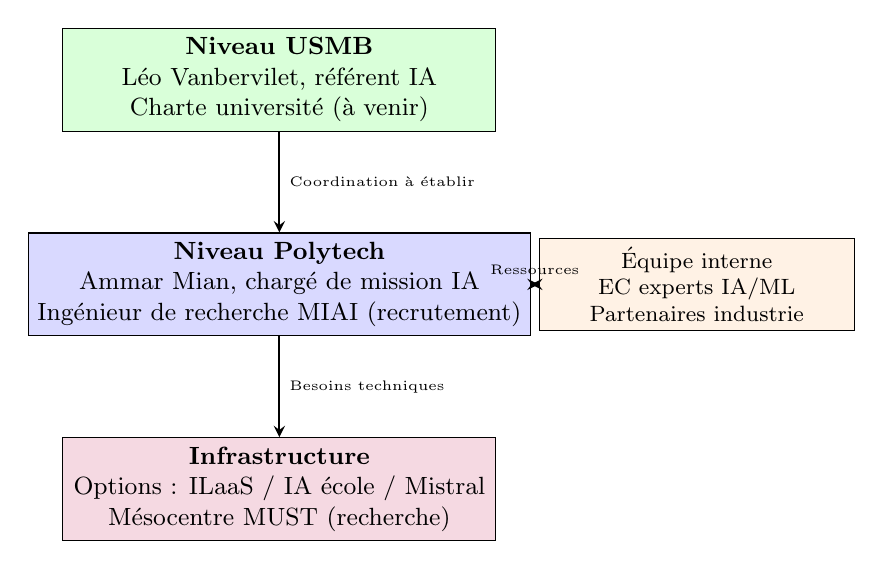
\begin{tikzpicture}[
  node distance=1.8cm,
  box/.style={rectangle, draw, fill=blue!10, minimum width=5.5cm, minimum height=1.2cm, font=\small, align=center},
  smallbox/.style={rectangle, draw, fill=orange!10, minimum width=4cm, minimum height=1cm, font=\footnotesize, align=center},
  arrow/.style={->, thick, >=stealth}
]
  % Niveau USMB (haut)
  \node[box, fill=green!15] (usmb) {\textbf{Niveau USMB}\\Léo Vanbervilet, référent IA\\Charte université (à venir)};

  % Niveau Polytech (milieu)
  \node[box, below of=usmb, yshift=-0.8cm, fill=blue!15] (polytech) {\textbf{Niveau Polytech}\\Ammar Mian, chargé de mission IA\\Ingénieur de recherche MIAI (recrutement)};

  % Niveau Infrastructure (bas)
  \node[box, below of=polytech, yshift=-0.8cm, fill=purple!15] (infra) {\textbf{Infrastructure}\\Options : ILaaS / IA école / Mistral\\Mésocentre MUST (recherche)};

  % Acteurs internes (côté)
  \node[smallbox, right of=polytech, xshift=3.5cm] (equipe) {Équipe interne\\EC experts IA/ML\\Partenaires industrie};

  % Flèches
  \draw[arrow] (usmb) -- (polytech) node[midway, right, font=\tiny, text width=2.5cm] {Coordination à établir};
  \draw[arrow] (polytech) -- (infra) node[midway, right, font=\tiny, text width=2cm] {Besoins techniques};
  \draw[arrow, dashed] (polytech) -- (equipe) node[midway, above, font=\tiny] {Ressources};
  \draw[arrow, dashed] (equipe) -- (polytech);

\end{tikzpicture}
\caption{Organisation IA actuelle et projetée pour Polytech Annecy-Chambéry}
\label{fig:gouvernance_coordonnee}
\end{figure}

Polytech Annecy-Chambéry dispose désormais d'une structuration \gls{ia} naissante : un chargé de mission dédié, un ingénieur de recherche en cours de recrutement, et une coordination à établir avec le référent \gls{usmb}. La stratégie retenue privilégie l'attente de la charte universitaire pour adaptation locale, l'exploration des options d'infrastructure technique, et une formation interne mobilisant les compétences existantes. Cette approche sobre et pragmatique permet d'avancer sans attendre des moyens budgétaires conséquents.

Au-delà de cette organisation, quelles recommandations transversales concrètes s'imposent ? Comment articuler formation des étudiants, adaptation des évaluations, accompagnement des enseignants et déploiement d'infrastructures souveraines dans une vision cohérente ? La section suivante formule ces recommandations opérationnelles~\cite{pascal2025ia}.
